\begin{figure}[!h] 
  \begin{subfigure}[b]{0.24\linewidth}
		\centering
		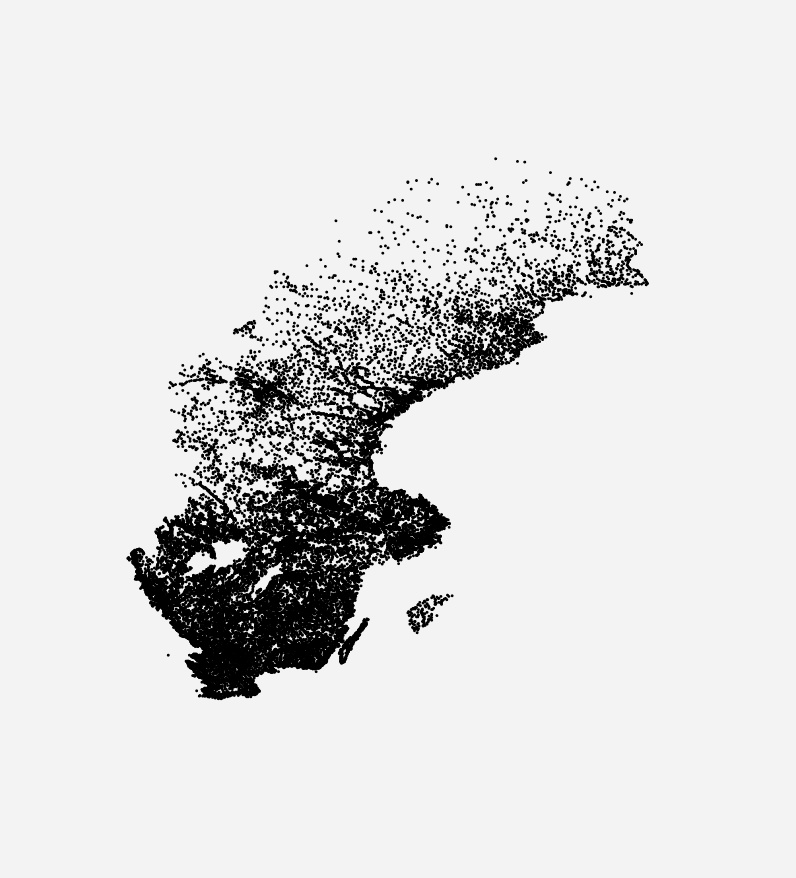
\includegraphics[width=0.9\linewidth]{Pictures/sweden} 
		\caption{\small Original Set} 
		\label{fig:or_sweden} 
		\vspace{4ex}
  \end{subfigure}
  \begin{subfigure}[b]{0.24\linewidth}
    \centering
    
\includegraphics[width=0.9\linewidth]{Pictures/10_sweden} 
	\caption{\small $d=10\%$} 
    \label{fig:10_sweden} 
    \vspace{4ex}
  \end{subfigure}%% 
  \begin{subfigure}[b]{0.24\linewidth}
    \centering
    
\includegraphics[width=0.9\linewidth]{Pictures/15_sweden} 
    \caption{\small $d=15\%$} 
    \label{fig:15_sweden} 
    \vspace{4ex}
  \end{subfigure}
  \begin{subfigure}[b]{0.24\linewidth}
  	\centering
  	
\includegraphics[width=0.9\linewidth]{Pictures/20_sweden} 
  	\caption{\small $d=20\%$} 
  	\label{fig:20_sweden} 
  	\vspace{4ex}
  \end{subfigure}
  \caption[Selected subsets from both graph building algorithms]{Selected subsets from both graph building algorithms. The points are selected starting from green to red. The data was obtained from the \href{http://www.math.uwaterloo.ca/tsp/world/swpoints.html}{University of Waterloo, Ontario, Canada}\cite{waterloo_sweden}.}
  \label{fig:sweden_dist} 
\end{figure}

